\documentclass[floatsintext,mask,man]{apa6}

\usepackage{amssymb,amsmath}
\usepackage{ifxetex,ifluatex}
\usepackage{fixltx2e} % provides \textsubscript
\ifnum 0\ifxetex 1\fi\ifluatex 1\fi=0 % if pdftex
  \usepackage[T1]{fontenc}
  \usepackage[utf8]{inputenc}
\else % if luatex or xelatex
  \ifxetex
    \usepackage{mathspec}
    \usepackage{xltxtra,xunicode}
  \else
    \usepackage{fontspec}
  \fi
  \defaultfontfeatures{Mapping=tex-text,Scale=MatchLowercase}
  \newcommand{\euro}{€}
\fi
% use upquote if available, for straight quotes in verbatim environments
\IfFileExists{upquote.sty}{\usepackage{upquote}}{}
% use microtype if available
\IfFileExists{microtype.sty}{\usepackage{microtype}}{}

% Table formatting
\usepackage{longtable, booktabs}
\usepackage{lscape}
% \usepackage[counterclockwise]{rotating}   % Landscape page setup for large tables
\usepackage{multirow}		% Table styling
\usepackage{tabularx}		% Control Column width
\usepackage[flushleft]{threeparttable}	% Allows for three part tables with a specified notes section
\usepackage{threeparttablex}            % Lets threeparttable work with longtable

% Create new environments so endfloat can handle them
% \newenvironment{ltable}
%   {\begin{landscape}\begin{center}\begin{threeparttable}}
%   {\end{threeparttable}\end{center}\end{landscape}}

\newenvironment{lltable}
  {\begin{landscape}\begin{center}\begin{ThreePartTable}}
  {\end{ThreePartTable}\end{center}\end{landscape}}




% The following enables adjusting longtable caption width to table width
% Solution found at http://golatex.de/longtable-mit-caption-so-breit-wie-die-tabelle-t15767.html
\makeatletter
\newcommand\LastLTentrywidth{1em}
\newlength\longtablewidth
\setlength{\longtablewidth}{1in}
\newcommand\getlongtablewidth{%
 \begingroup
  \ifcsname LT@\roman{LT@tables}\endcsname
  \global\longtablewidth=0pt
  \renewcommand\LT@entry[2]{\global\advance\longtablewidth by ##2\relax\gdef\LastLTentrywidth{##2}}%
  \@nameuse{LT@\roman{LT@tables}}%
  \fi
\endgroup}


\ifxetex
  \usepackage[setpagesize=false, % page size defined by xetex
              unicode=false, % unicode breaks when used with xetex
              xetex]{hyperref}
\else
  \usepackage[unicode=true]{hyperref}
\fi
\hypersetup{breaklinks=true,
            pdfauthor={},
            pdftitle={Polite speech emerges from competing social goals},
            colorlinks=true,
            citecolor=blue,
            urlcolor=blue,
            linkcolor=black,
            pdfborder={0 0 0}}
\urlstyle{same}  % don't use monospace font for urls

\setlength{\parindent}{0pt}
%\setlength{\parskip}{0pt plus 0pt minus 0pt}

\setlength{\emergencystretch}{3em}  % prevent overfull lines


% Manuscript styling
\captionsetup{font=singlespacing,justification=justified}
\usepackage{csquotes}
\usepackage{upgreek}

 % Line numbering
  \usepackage{lineno}
  \linenumbers


\usepackage{tikz} % Variable definition to generate author note

% fix for \tightlist problem in pandoc 1.14
\providecommand{\tightlist}{%
  \setlength{\itemsep}{0pt}\setlength{\parskip}{0pt}}

% Essential manuscript parts
  \title{Polite speech emerges from competing social goals}

  \shorttitle{Modeling polite speech}


  \author{Erica J. Yoon\textsuperscript{1, *, †}, Michael Henry Tessler\textsuperscript{1, †}, Noah D. Goodman\textsuperscript{1}, \& Michael C. Frank\textsuperscript{1}}

  % \def\affdep{{"", "", "", ""}}%
  % \def\affcity{{"", "", "", ""}}%

  \affiliation{
    \vspace{0.5cm}
          \textsuperscript{1} Department of Psychology, Stanford University\\
          \textsuperscript{*} Corresponding author\\
          \textsuperscript{†} These authors contributed equally to this work.  }

  \authornote{
    Correspondence concerning this article should be addressed to Erica J.
    Yoon, 450 Serra Mall, Bldg. 420, Rm. 290, Stanford, CA 94305. E-mail:
    \href{mailto:ejyoon@stanford.edu}{\nolinkurl{ejyoon@stanford.edu}}
  }


  \abstract{Language is a remarkably efficient tool for information transfer. Yet to
be polite, speakers often behave in ways that are at odds with this
goal, making statements that are inefficient, imprecise, or even
outright false. Why? We show that polite speech emerges from competing
goals: to be informative, to be kind, and to \emph{appear} to be both of
these. We formalize this tradeoff using a probabilistic model of
speakers' utterance choice, which predicts human judg- ments with high
accuracy. This utility-theoretic approach to speech acts takes a step
towards explaining the richness and subtlety of social language.}
  \keywords{Politeness; computational modeling; commmunicative goals; pragmatics \\

    \indent Word count: 3500
  }





\usepackage{amsthm}
\newtheorem{theorem}{Theorem}
\newtheorem{lemma}{Lemma}
\theoremstyle{definition}
\newtheorem{definition}{Definition}
\newtheorem{corollary}{Corollary}
\newtheorem{proposition}{Proposition}
\theoremstyle{definition}
\newtheorem{example}{Example}
\theoremstyle{definition}
\newtheorem{exercise}{Exercise}
\theoremstyle{remark}
\newtheorem*{remark}{Remark}
\newtheorem*{solution}{Solution}
\begin{document}

\maketitle

\setcounter{secnumdepth}{0}



\definecolor{Blue}{RGB}{10,100,200} \definecolor{Red}{RGB}{255,0,0}

\newcommand{\red}[1]{{\textcolor{Red}{#1}}}
\newcommand{\mht}[1]{{\textcolor{Blue}{[mht: #1]}}}





















\section{Supplementary Information}\label{supplementary-information}

\subsection{Data analysis}\label{data-analysis}

We used R (Version 3.4.3; R Core Team, 2017) and the R-packages
\emph{BayesFactor} (Version 0.9.12.2; Morey \& Rouder, 2015),
\emph{bindrcpp} (Version 0.2; Müller, 2017a), \emph{binom} (Version
1.1.1; Dorai-Raj, 2014), \emph{brms} (Version 2.0.1; Bürkner, 2017),
\emph{coda} (Version 0.19.1; Plummer, Best, Cowles, \& Vines, 2006),
\emph{directlabels} (Version 2017.3.31; Hocking, 2017), \emph{dplyr}
(Version 0.7.4; Wickham, Francois, Henry, \& Müller, 2017),
\emph{forcats} (Version 0.2.0; Wickham, 2017a), \emph{ggplot2} (Version
2.2.1; Wickham, 2009), \emph{ggthemes} (Version 3.4.0; Arnold, 2017),
\emph{gridExtra} (Version 2.3; Auguie, 2017), \emph{here} (Version 0.1;
Müller, 2017b), \emph{jsonlite} (Version 1.5; Ooms, 2014),
\emph{langcog} (Version 0.1.9001; Braginsky, Yurovsky, \& Frank, n.d.),
\emph{lme4} (Version 1.1.15; Bates, Mächler, Bolker, \& Walker, 2015),
\emph{magrittr} (Version 1.5; Bache \& Wickham, 2014), \emph{Matrix}
(Version 1.2.12; Bates \& Maechler, 2017), \emph{papaja} (Version
0.1.0.9655; Aust \& Barth, 2017), \emph{purrr} (Version 0.2.4; Henry \&
Wickham, 2017), \emph{RColorBrewer} (Version 1.1.2; Neuwirth, 2014),
\emph{Rcpp} (Eddelbuettel \& Balamuta, 2017; Version 0.12.17;
Eddelbuettel \& François, 2011), \emph{readr} (Version 1.1.1; Wickham,
Hester, \& Francois, 2017), \emph{rwebppl} (Version 0.1.97; Braginsky,
Tessler, \& Hawkins, n.d.), \emph{stringr} (Version 1.3.1; Wickham,
2017b), \emph{tibble} (Version 1.4.2; Müller \& Wickham, 2017),
\emph{tidyr} (Version 0.7.2; Wickham \& Henry, 2017), and
\emph{tidyverse} (Version 1.2.1; Wickham, 2017c) for all our analyses.

\subsection{Full statistics on human
data}\label{full-statistics-on-human-data}

\begin{table}[tbp]
\begin{center}
\begin{threeparttable}
\caption{\label{tab:brmTab}Predictor mean estimates with standard deviation and 95\% credible interval information for a Bayesian linear mixed-effects model predicting negation production based on true state and speaker goal (with both-goal as the reference level).}
\begin{tabular}{lllll}
\toprule
Predictor & \multicolumn{1}{c}{Mean} & \multicolumn{1}{c}{SD} & \multicolumn{1}{c}{95\% CI-Lower} & \multicolumn{1}{c}{95\% CI-Upper}\\
\midrule
Intercept & 0.88 & 0.13 & 0.63 & 1.12\\
True state & 2.18 & 0.17 & 1.86 & 2.53\\
Goal: Informative & 0.47 & 0.17 & 0.14 & 0.80\\
Goal: Kind & 0.97 & 0.25 & 0.51 & 1.49\\
True state * Informative & -1.33 & 0.18 & -1.69 & -0.98\\
True state * Kind & -0.50 & 0.22 & -0.92 & -0.07\\
\bottomrule
\end{tabular}
\end{threeparttable}
\end{center}
\end{table}

We used Bayesian linear mixed-effects models (\texttt{brms} package in
R; Bürkner, 2017) using crossed random effects of true state and goal
with maximal random effects structure (Barr, Levy, Scheepers, \& Tily,
2013; Gelman \& Hill, 2006).

\subsection{Model fitting and inferred
parameters}\label{model-fitting-and-inferred-parameters}

\begin{table}[tbp]
\begin{center}
\begin{threeparttable}
\caption{\label{tab:otherParams}Inferred negation cost and speaker optimality parameters for all model variants.}
\begin{tabular}{lll}
\toprule
Model & \multicolumn{1}{c}{Cost of negation} & \multicolumn{1}{c}{Speaker optimality}\\
\midrule
informational only & 1.58 & 8.58\\
informational, presentational & 1.89 & 2.93\\
informational, social & 1.11 & 3.07\\
informational, social, presentational & 2.64 & 4.47\\
presentational only & 2.58 & 9.58\\
social only & 1.73 & 7.23\\
social, presentational & 2.49 & 5.29\\
\bottomrule
\end{tabular}
\end{threeparttable}
\end{center}
\end{table}

In the speaker production task, participants were told the speakers'
intentions (e.g., wanted to make Bob feel good). We assume that the
intention descriptions conveyed some mixture of weights \(\phi_{epi}\),
\(\phi_{soc}\), \(\phi_{pres}\), and \(\phi_{S_1}\) that the speaker was
using. We put uninformative priors on the unnormalized mixture weights
(\(\phi\) \textasciitilde{} \(Uniform(0,1)\)) separately for each goal
condition (\enquote{wanted to be X}; \emph{kind}, \emph{informative}, or
\emph{both}). In addition, the full model has two global parameters: the
speaker's soft-max parameter \(\lambda_{S_2}\) and soft-max paramater of
the hypothetical speaker that the pragmatic listener reasons about
\(\lambda_{S_1}\). \(\lambda_{S_1}\) was 1, and \(\lambda_{S_2}\) was
inferred from the data: We put a prior that was consistent with those
used for similar models in this model class: \(\lambda_{S_2}\)
\textasciitilde{} \(Uniform(0,20)\). Finally, we incorporate the literal
semantics data into the RSA model by maintaining uncertainty about the
semantic weight of utterance \(w\) for state \(s\), for each of the
states and utterances, and assuming a Beta-Binomial linking function
between these weights and the literal semantics data (see \emph{Literal
semantics task} above). We infer the posterior distribution over all of
the model parameters and generate model predictions based on this
posterior distribution using Bayesian data analysis (Lee \& Wagenmakers,
2014). We ran 4 MCMC chains for 80,000 iterations, discarding the first
40,000 for burnin. Negation cost and speaker optimality parameters are
shown in Table \ref{tab:otherParams}.

\newpage

\subsection{Supplemental Figures}\label{supplemental-figures}

\begin{figure}[!h]
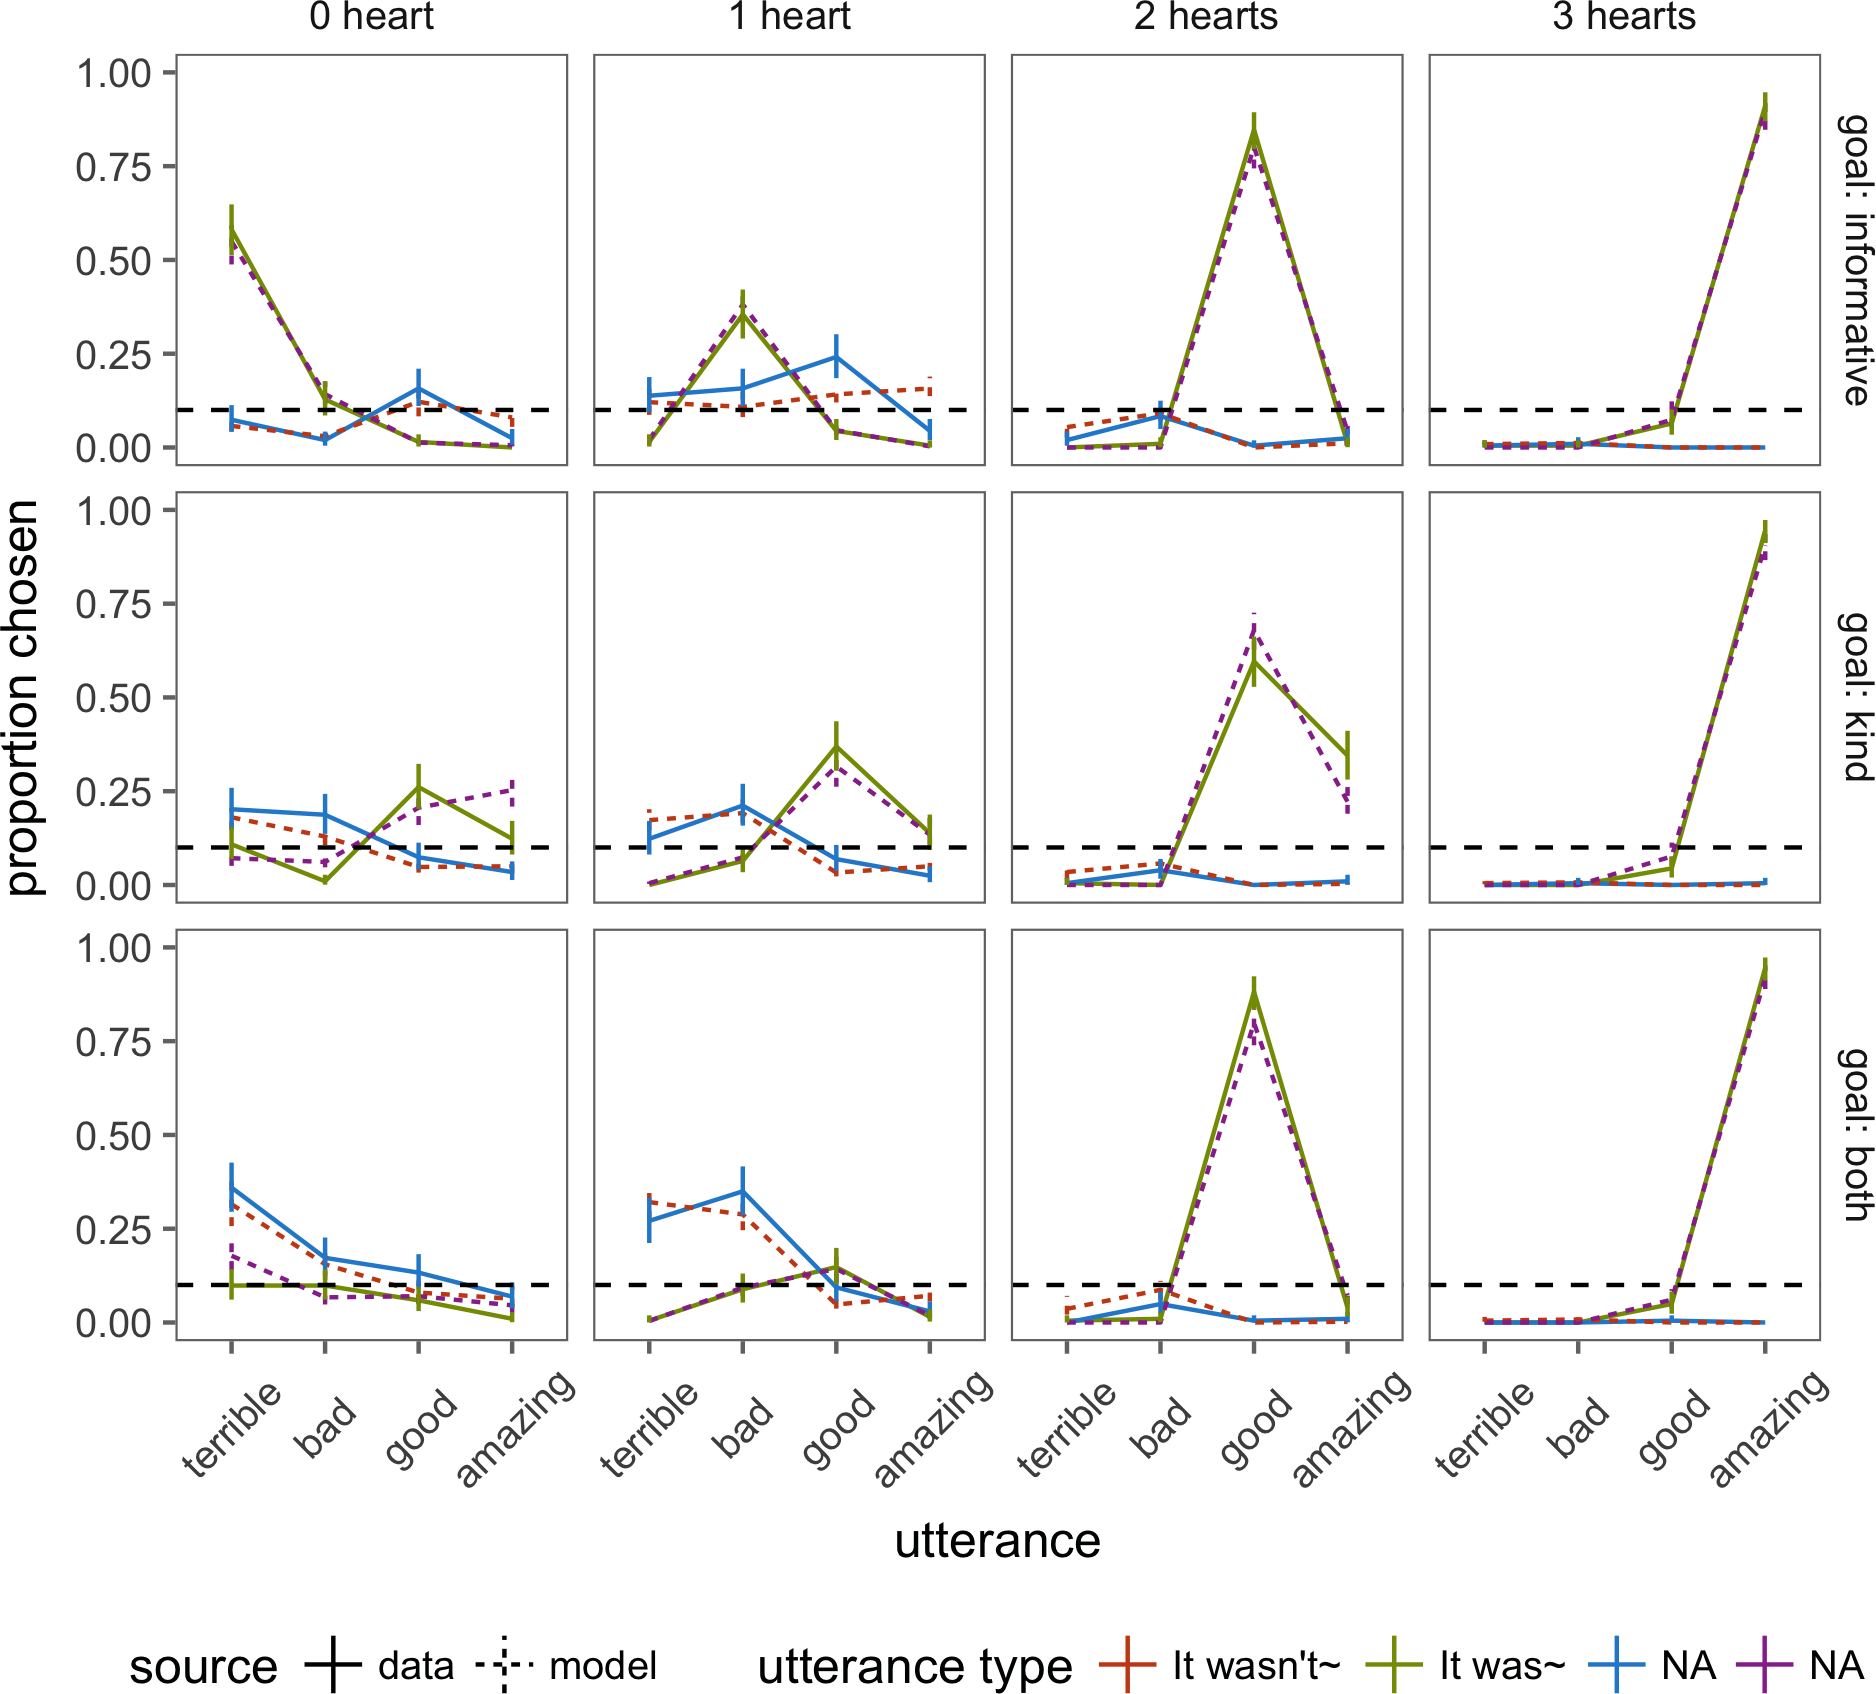
\includegraphics[width=\textwidth]{polite_NHB_anonymous_supp_files/figure-latex/utterance-1} \caption{Experimental results (solid lines) and fitted predictions from the full model (dashed lines) for speaker production. Proportion of utterances chosen (utterance type – direct vs. indirect – in different colors and words shown on x-axis) given the true states (columns) and speaker goals (rows). Error bars represent 95\% confidence intervals for the data and 95\% highest density intervals for the model. Black dotted line represents the chance level.}\label{fig:utterance}
\end{figure}

\begin{figure}[!h]
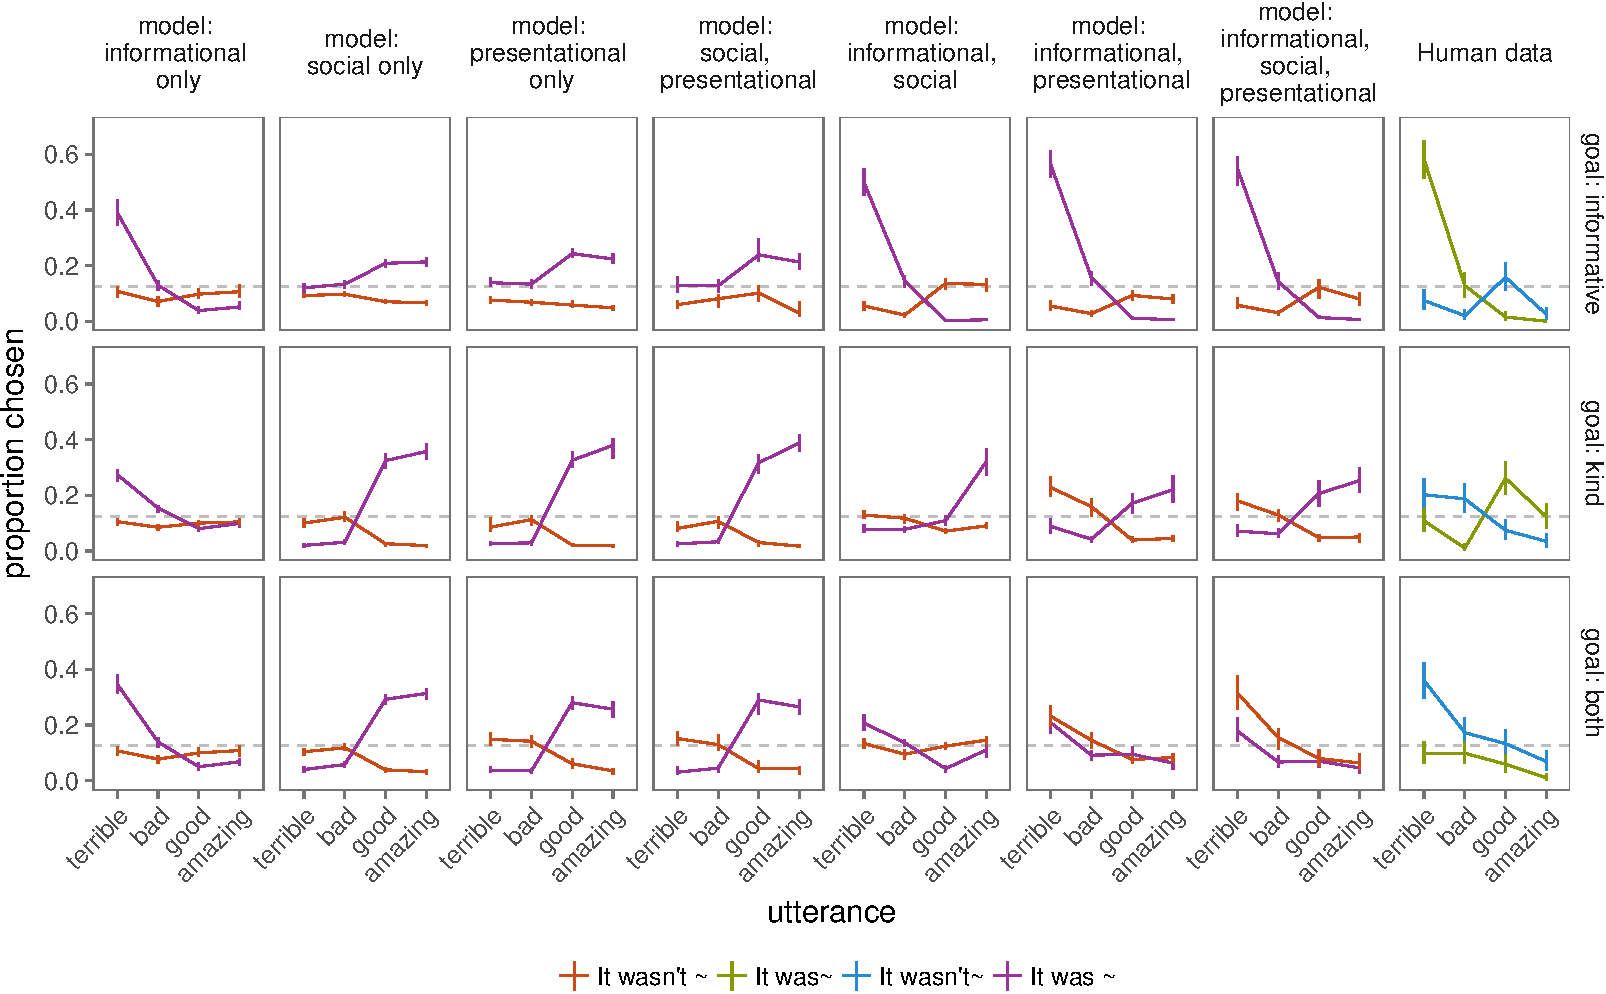
\includegraphics[width=\textwidth]{polite_NHB_anonymous_supp_files/figure-latex/comparisonAll-1} \caption{Comparison of predictions for proportion of utterances chosen by pragmatic speaker from possible model variants (left) and human data (rightmost) for average proportion of negation produced among all utterances, given true state of 0 heart and speaker with a goal to be informative (top), kind (middle), or both (bottom). Gray dotted line indicates chance level at 12.5\%.}\label{fig:comparisonAll}
\end{figure}

\begin{figure}[!h]
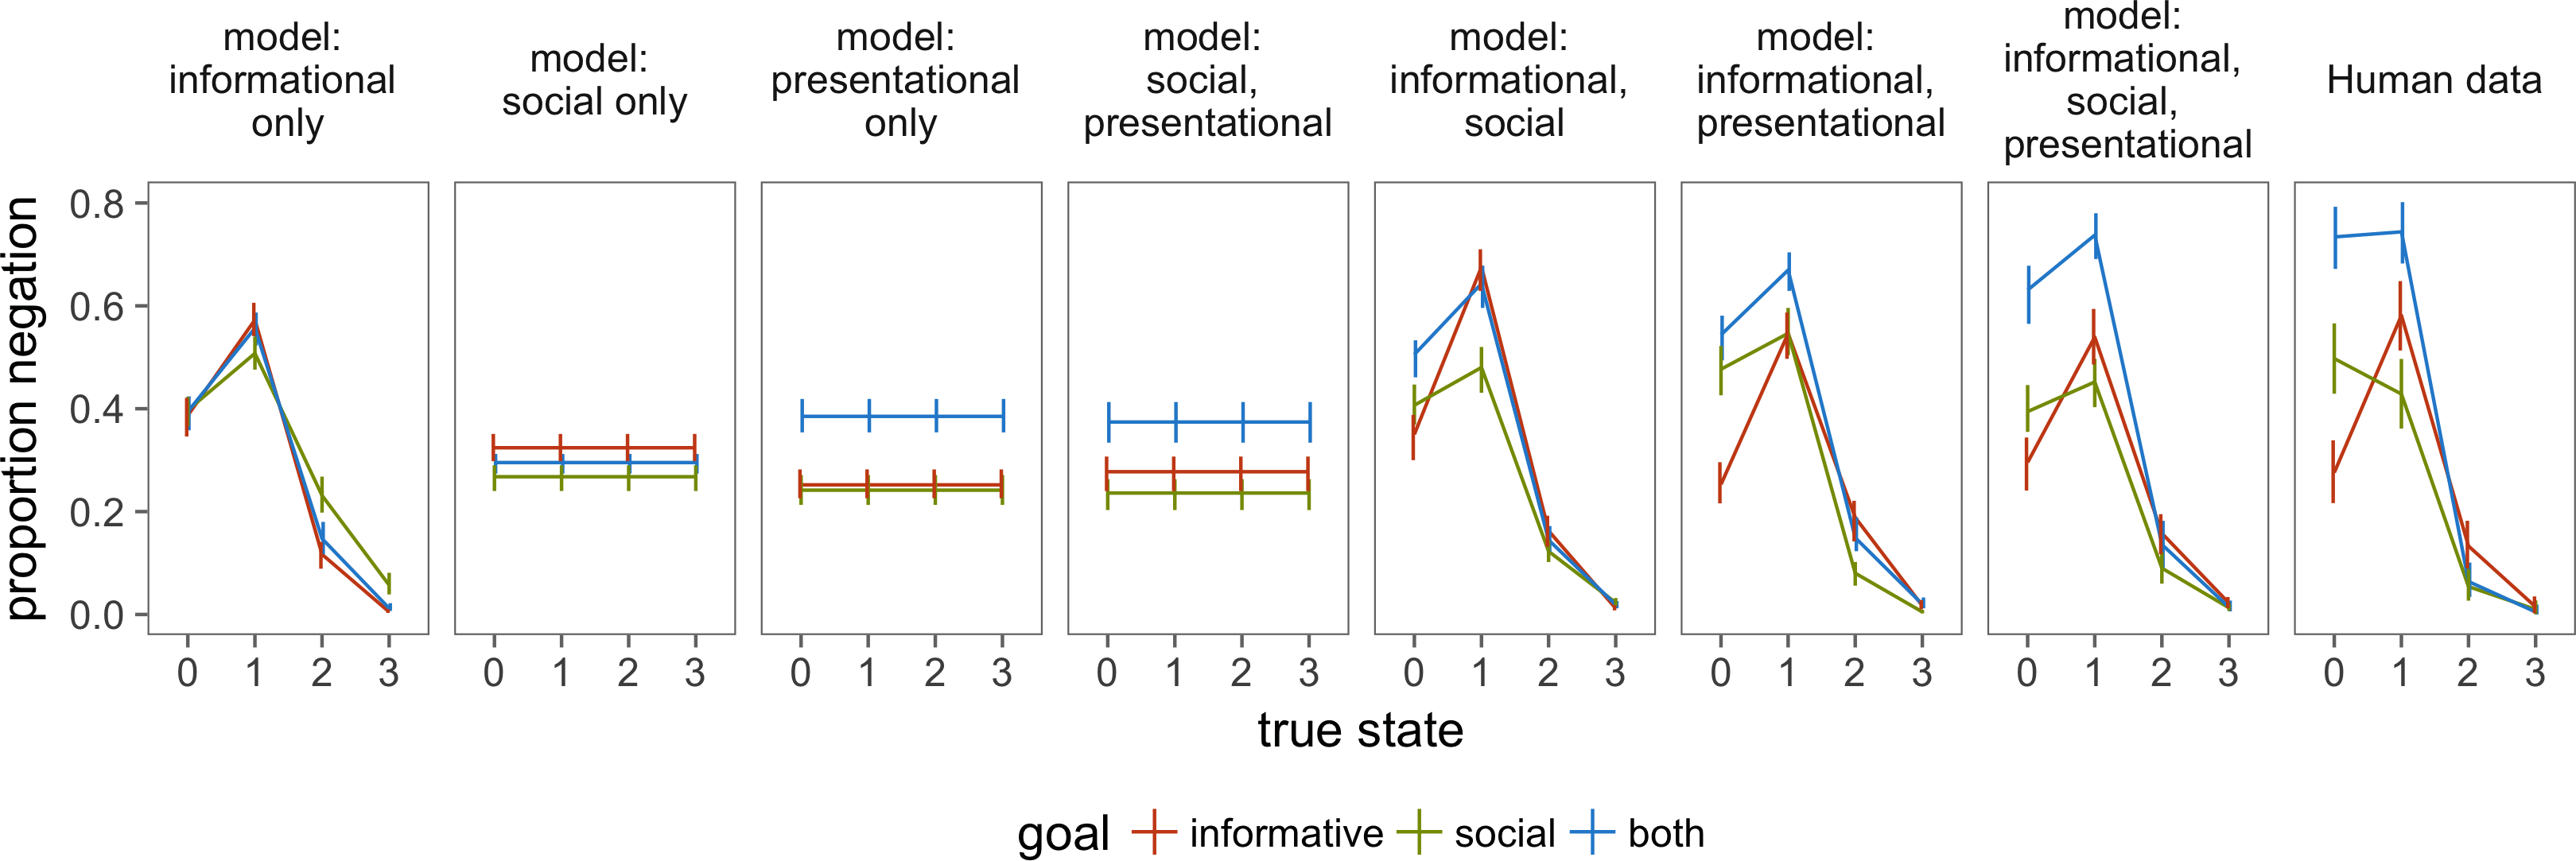
\includegraphics[width=\textwidth]{polite_NHB_anonymous_supp_files/figure-latex/negation-1} \caption{Experimental results (left) and fitted model predictions (right) for average proportion of negation produced among all utterances, given true states (x-axis) and goals (colors).}\label{fig:negation}
\end{figure}

\newpage

\section{References}\label{references}

\setlength{\parindent}{-0.5in} \setlength{\leftskip}{0.5in}

\hypertarget{refs}{}
\hypertarget{ref-R-ggthemes}{}
Arnold, J. B. (2017). \emph{Ggthemes: Extra themes, scales and geoms for
'ggplot2'}. Retrieved from
\url{https://CRAN.R-project.org/package=ggthemes}

\hypertarget{ref-R-gridExtra}{}
Auguie, B. (2017). \emph{GridExtra: Miscellaneous functions for ``grid''
graphics}. Retrieved from
\url{https://CRAN.R-project.org/package=gridExtra}

\hypertarget{ref-R-papaja}{}
Aust, F., \& Barth, M. (2017). \emph{papaja: Create APA manuscripts with
R Markdown}. Retrieved from \url{https://github.com/crsh/papaja}

\hypertarget{ref-R-magrittr}{}
Bache, S. M., \& Wickham, H. (2014). \emph{Magrittr: A forward-pipe
operator for r}. Retrieved from
\url{https://CRAN.R-project.org/package=magrittr}

\hypertarget{ref-barr2013random}{}
Barr, D. J., Levy, R., Scheepers, C., \& Tily, H. J. (2013). Random
effects structure for confirmatory hypothesis testing: Keep it maximal.
\emph{Journal of Memory and Language}, \emph{68}(3), 255--278.

\hypertarget{ref-R-Matrix}{}
Bates, D., \& Maechler, M. (2017). \emph{Matrix: Sparse and dense matrix
classes and methods}. Retrieved from
\url{https://CRAN.R-project.org/package=Matrix}

\hypertarget{ref-R-lme4}{}
Bates, D., Mächler, M., Bolker, B., \& Walker, S. (2015). Fitting linear
mixed-effects models using lme4. \emph{Journal of Statistical Software},
\emph{67}(1), 1--48.
doi:\href{https://doi.org/10.18637/jss.v067.i01}{10.18637/jss.v067.i01}

\hypertarget{ref-R-rwebppl}{}
Braginsky, M., Tessler, M. H., \& Hawkins, R. (n.d.). \emph{Rwebppl: R
interface to webppl}. Retrieved from
\url{https://github.com/mhtess/rwebppl}

\hypertarget{ref-R-langcog}{}
Braginsky, M., Yurovsky, D., \& Frank, M. C. (n.d.). \emph{Langcog:
Language and cognition lab things}. Retrieved from
\url{http://github.com/langcog/langcog}

\hypertarget{ref-R-brms}{}
Bürkner, P.-C. (2017). brms: An R package for bayesian multilevel models
using Stan. \emph{Journal of Statistical Software}, \emph{80}(1), 1--28.
doi:\href{https://doi.org/10.18637/jss.v080.i01}{10.18637/jss.v080.i01}

\hypertarget{ref-R-binom}{}
Dorai-Raj, S. (2014). \emph{Binom: Binomial confidence intervals for
several parameterizations}. Retrieved from
\url{https://CRAN.R-project.org/package=binom}

\hypertarget{ref-R-Rcpp_b}{}
Eddelbuettel, D., \& Balamuta, J. J. (2017). Extending extitR with
extitC++: A Brief Introduction to extitRcpp. \emph{PeerJ Preprints},
\emph{5}, e3188v1.
doi:\href{https://doi.org/10.7287/peerj.preprints.3188v1}{10.7287/peerj.preprints.3188v1}

\hypertarget{ref-R-Rcpp_a}{}
Eddelbuettel, D., \& François, R. (2011). Rcpp: Seamless R and C++
integration. \emph{Journal of Statistical Software}, \emph{40}(8),
1--18.
doi:\href{https://doi.org/10.18637/jss.v040.i08}{10.18637/jss.v040.i08}

\hypertarget{ref-gelman2006data}{}
Gelman, A., \& Hill, J. (2006). \emph{Data analysis using regression and
multilevel/hierarchical models}. Cambridge university press.

\hypertarget{ref-R-purrr}{}
Henry, L., \& Wickham, H. (2017). \emph{Purrr: Functional programming
tools}. Retrieved from \url{https://CRAN.R-project.org/package=purrr}

\hypertarget{ref-R-directlabels}{}
Hocking, T. D. (2017). \emph{Directlabels: Direct labels for multicolor
plots}. Retrieved from
\url{https://CRAN.R-project.org/package=directlabels}

\hypertarget{ref-lee2014}{}
Lee, M. D., \& Wagenmakers, E. J. (2014). \emph{Bayesian cognitive
modeling: A practical course}. Cambridge Univ. Press.

\hypertarget{ref-R-BayesFactor}{}
Morey, R. D., \& Rouder, J. N. (2015). \emph{BayesFactor: Computation of
bayes factors for common designs}. Retrieved from
\url{https://CRAN.R-project.org/package=BayesFactor}

\hypertarget{ref-R-bindrcpp}{}
Müller, K. (2017a). \emph{Bindrcpp: An 'rcpp' interface to active
bindings}. Retrieved from
\url{https://CRAN.R-project.org/package=bindrcpp}

\hypertarget{ref-R-here}{}
Müller, K. (2017b). \emph{Here: A simpler way to find your files}.
Retrieved from \url{https://CRAN.R-project.org/package=here}

\hypertarget{ref-R-tibble}{}
Müller, K., \& Wickham, H. (2017). \emph{Tibble: Simple data frames}.
Retrieved from \url{https://CRAN.R-project.org/package=tibble}

\hypertarget{ref-R-RColorBrewer}{}
Neuwirth, E. (2014). \emph{RColorBrewer: ColorBrewer palettes}.
Retrieved from \url{https://CRAN.R-project.org/package=RColorBrewer}

\hypertarget{ref-R-jsonlite}{}
Ooms, J. (2014). The jsonlite package: A practical and consistent
mapping between json data and r objects. \emph{arXiv:1403.2805
{[}Stat.CO{]}}. Retrieved from \url{https://arxiv.org/abs/1403.2805}

\hypertarget{ref-R-coda}{}
Plummer, M., Best, N., Cowles, K., \& Vines, K. (2006). CODA:
Convergence diagnosis and output analysis for mcmc. \emph{R News},
\emph{6}(1), 7--11. Retrieved from
\url{https://journal.r-project.org/archive/}

\hypertarget{ref-R-base}{}
R Core Team. (2017). \emph{R: A language and environment for statistical
computing}. Vienna, Austria: R Foundation for Statistical Computing.
Retrieved from \url{https://www.R-project.org/}

\hypertarget{ref-R-ggplot2}{}
Wickham, H. (2009). \emph{Ggplot2: Elegant graphics for data analysis}.
Springer-Verlag New York. Retrieved from \url{http://ggplot2.org}

\hypertarget{ref-R-forcats}{}
Wickham, H. (2017a). \emph{Forcats: Tools for working with categorical
variables (factors)}. Retrieved from
\url{https://CRAN.R-project.org/package=forcats}

\hypertarget{ref-R-stringr}{}
Wickham, H. (2017b). \emph{Stringr: Simple, consistent wrappers for
common string operations}. Retrieved from
\url{https://CRAN.R-project.org/package=stringr}

\hypertarget{ref-R-tidyverse}{}
Wickham, H. (2017c). \emph{Tidyverse: Easily install and load the
'tidyverse'}. Retrieved from
\url{https://CRAN.R-project.org/package=tidyverse}

\hypertarget{ref-R-tidyr}{}
Wickham, H., \& Henry, L. (2017). \emph{Tidyr: Easily tidy data with
'spread()' and 'gather()' functions}. Retrieved from
\url{https://CRAN.R-project.org/package=tidyr}

\hypertarget{ref-R-dplyr}{}
Wickham, H., Francois, R., Henry, L., \& Müller, K. (2017). \emph{Dplyr:
A grammar of data manipulation}. Retrieved from
\url{https://CRAN.R-project.org/package=dplyr}

\hypertarget{ref-R-readr}{}
Wickham, H., Hester, J., \& Francois, R. (2017). \emph{Readr: Read
rectangular text data}. Retrieved from
\url{https://CRAN.R-project.org/package=readr}






\end{document}
